
%!TEX root = ../thesis.tex
%*******************************************************************************
%****************************** Third Chapter **********************************
%*******************************************************************************
\chapter{Simulating and Reconstructing SBND}
\label{Chapter6}

% **************************** Define Graphics Path **************************
\ifpdf
    \graphicspath{{Chapter6/Figs/Raster/}{Chapter6/Figs/PDF/}{Chapter6/Figs/}}
\else
    \graphicspath{{Chapter6/Figs/Vector/}{Chapter6/Figs/}}
\fi

%********************************** %Opening  **************************************

Chapter 6 Opening

\newpage

%********************************** %First Section  **************************************
\section{Simulating SBND}

%Modern physics experiments and MC
Many modern physics experiments heavily relies on simulations to develop reconstruction and analysis tools, as well as to understand the physics capabilities of the detector.
Monte Carlo (MC) simulations is the most general and widely used method that use random sampling from a predefined distributions. 
At SBND, the workflow for simulation and reconstruction is provided by the LArSoft framework \cite{}, which has been employed by many other LArTPC experiments.
This framework enables sharing common simulation, reconstruction and analysis tools across collaborations including ArgoNeuT, MicroBooNE, DUNE, SBND and ICARUS.

%Describe the overall workflow
An overview of the simulation workflow is depicted in Fig. \ref{fig:Sim_Workflow}.
The process begins with a generator to produce primary particles that enter the detector, shown by the purple box.
The primary particles can be neutrinos, cosmic muons or BSM particles depending on the type of generator.
The propagation of the primary particle inside and outside the detector, and the resulting energy deposition is simulated using Geant4 \cite{}, shown by the green boxes.
For interactions inside the detector, the charge and light yield is calculated from the energy deposition.
The number of ionisation electrons from charge yield are propagated through the detector to the wire planes using Wirecell \cite{}, shown by the red boxes.
The number of scintillation photons from light yield are propagating to the photodetectors using a semi-analytical light library \cite{}, shown by the blue boxes.
For interactions outside of the detector, only the energy depositions within the CRT strips is converted into light yield, shown by the orange box.
The detector response is then simulated for each detector subsystem.
By the end of this stage, the waveforms from each subsystem ideally represent real data.

\begin{figure}[htbp!] 
\centering    
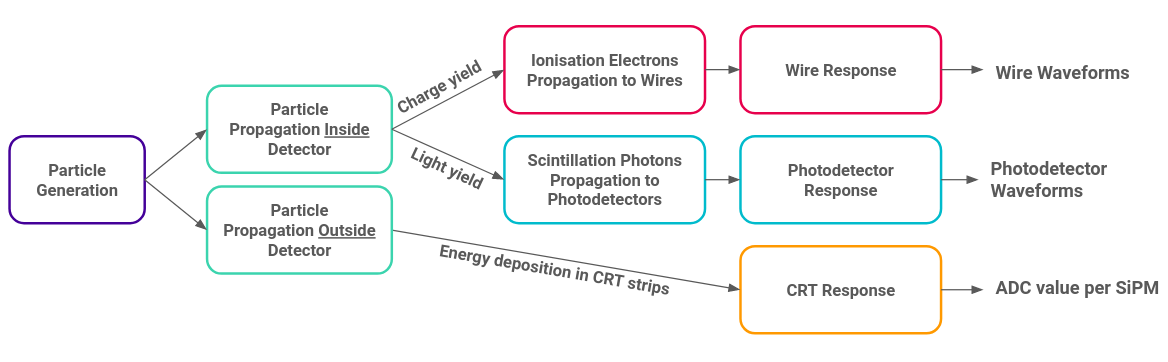
\includegraphics[width=1.0\textwidth]{Sim_Workflow}
\caption[Sim_Workflow]{
Overview of the workflow to simulate the SBND detector.
}
\label{fig:Sim_Workflow}
\end{figure}

The following section covers the simulation workflow for the SBND detector.
Sec. \ref{sec:gen_mevprtl}, \ref{sec:gen_genie} and \ref{sec:gen_corsika} provides the details of the three particle generators to simulate HNLs, neutrinos and cosmic muons respectively.
The simulation of the primary particle propagation using the Geant4 tool kit is outlined in Sec. \ref{sec:gen_g4}.
The propagation of the resulting ionisation electrons and scintillation photons to the respective detection subsystems and their responses are discussed in Sec. \ref{sec:gen_response}. 

%Introduce different types of event generator

\subsection{HNL Generator: MeVPrtl}
\label{sec:gen_mevprtl}

%MeVPrtl Workflow
HNLs are generated using the MeVPrtl generator \cite{}, which is joint effort by ICARUS and SBND collaborators towards a sharing BSM generator.
MeVPrtl was developed as a modular generator, allowing for easy adaptations for different beam sources and detectors, as well as direct interface with the existing LArSoft framework.
The workflow of the MeVPrtl is broken down into 4 stages, as illustrated in Fig. \ref{fig:MeVPrtl_Workflow}.
The generator begins with taking an input of meson fluxes, representing the particles produced from a beam source.
It then simulates the meson decaying to a BSM particle, which is propagated to the detector and decays back into a SM observable.
There are several BSM models already implemented in the MeVPrtl generator, including HNLs, Higgs portal scalars \cite{} and heavy QCD axions \cite{}.


\begin{figure}[htbp!] 
\centering    
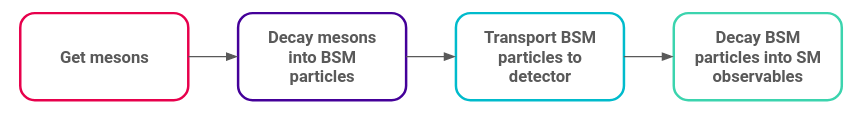
\includegraphics[width=1.0\textwidth]{MeVPrtl_Workflow}
\caption[MeVPrtl_Workflow]{
Overview of the workflow of the MeVPrtl generator.
}
\label{fig:MeVPrtl_Workflow}
\end{figure}

%Each stage validation
For the purpose of generating HNLs coming from the BNB, the generator begins with sampling the long-lived $K^{+}$ fluxes of the BNB, which is previously shown in Fig. \ref{fig:BNB_Meson_Flux}.
Instead of decaying into a SM neutrino, the kaons decay into a HNL, with branching ratio defined by Eq. \ref{eq:kaon_decay_hnl}.
The resulting HNL is then propagated to detector by ray forcing.
This method forces the HNL to hit the SBND detector by picking a direction that impinges the particle at the detector front face, and then calculates the probability of this direction. 
Then, the HNL decays back into the SM observables.
For example of the $\nu\pi^{0}$ final state, the decay width is defined by Eq. \ref{eq:pi0}.
The kinematics of the decay products is simulated for a Majorana HNL isotropically decays in the rest frame, and is subsequently boosted to the lab frame. 
The decay products are then propagated through the detector by Geant4, which will be described in the upcoming section.

%Timing
The key motivation of the HNL search is the timing delay between a HNL compared to a SM neutrino.  
The key implementation of this generator is the consistency of simulating the time of flight between the MeVPrtl generator for HNLs and the GENIE generator for SM neutrinos.


%Some truth distribution: Energy spectrum/ Daughter kinematics distribution/ Timing distribution


\subsection{Neutrino Generator: GENIE}
\label{sec:gen_genie}

%Overview of GENIE

%What kind of tune are being used

SM neutrino interactions are generated by the GENIE generator \cite{genie}, which provides a selection of theoretical and empirical models for different physic process.
These models can be combined into a \textit{tune} by comparing predictions to data from neutrino and electron scattering experiments.
The SBND collaboration is planning to use a tune that was specifically developed to serve as a baseline model for the SBN and DUNE oscillation analysis.
Details for the basis of the tune can be found in Table 1 in Ref. \cite{genie_tune}, with ongoing developments on the choice of models documented in Ref. \cite{genie_tune_github}.  

In general, GENIE first selects a nuclear model that describes the momenta and potential energy of the nucleons to model nuclear effects.
Then, the neutrino flux and the integrated cross section model are used to compute the probability if a neutrino interaction occurs.
The differential cross section is then used to determine the type of neutrino interaction and the kinematic range.
The neutrino interaction types include Quasi-Elastic (QE), Baryonic Resonant Scattering (RES), Coherent Scattering (COH), Deep Inelastic Scattering and $\nu$-e elastic scattering.
DIS interaction can additionally produce hadrons within the nuclei, of which these hadrons can propagate through the nucleus and modify the observed kinematics.
Thus, the choice of Final State Interaction (FSI) model is also crucially important for predicting the observable topology of neutrino interactions since argon is a heavy nuclear target.

In addition to the tune, the GENIE generator also provides a re-weighting scheme to evaluate the systematic uncertainties for a model chosen in the tune.
Due to the scarcity of neutrino interaction data, particularly for $\nu-Ar$ interaction, the uncertainties in cross section modelling tend to be large, and can hamper the capabilities of the HNL sensitivity.  
The neutrino interaction re-weighting scheme, and the resulting systematics uncertainties impact on the HNL search will be discussed in details in Sec. \ref{}.


GENIE simulates neutrino interactions occurring both inside and outside of the detector volume, with boundary defined in Fig. \ref{fig:Rockbox_Volume}.  
All interactions occurring inside the detector volume are strictly kept.
Outside of the detector, a buffer volume is defined as 5 m surrounding the detector volume.
An additional Rockbox volume is defined by extending the buffer volume backwards in the beam direction ($z$-axis) up to 15 m in front of the buffer volume.
Both these volumes are referred to together as the \textit{Rockbox} volume in this thesis.
Neutrino interactions within this volume are kept, whose products can potentially deposit energy in the detector.
These interactions are referred to as \textit{dirt} neutrinos, and constitute to a significant background to the HNL search.
The background rejection of dirt neutrinos will be covered in Sec. \ref{}.

\begin{figure}[htbp!] 
\centering    
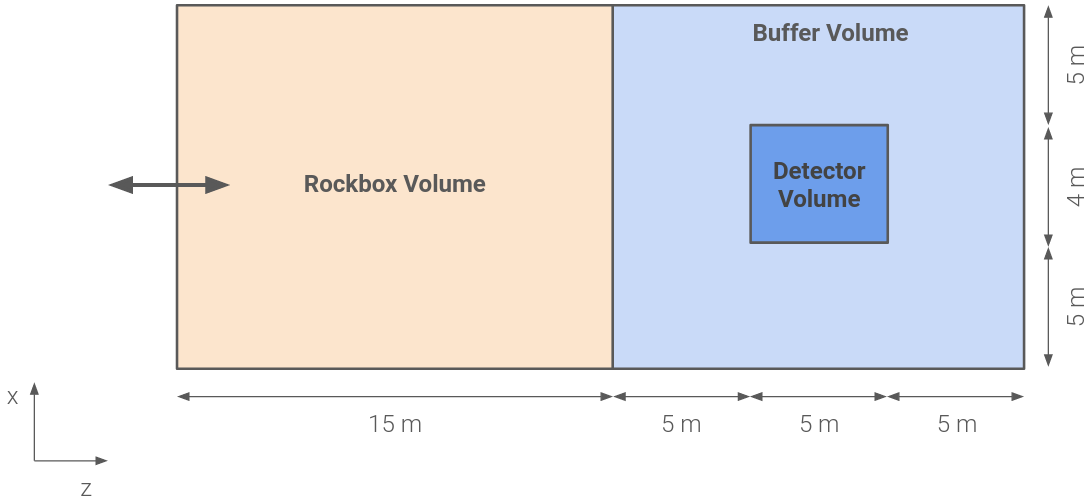
\includegraphics[width=0.85\textwidth]{Rockbox_Volume}
\caption[Rockbox_Volume]{
Diagram showing the volume boundary defined by the GENIE generator to simulate neutrino interactions occurring inside and outside of the detector volume. 
}
\label{fig:Rockbox_Volume}
\end{figure}

\subsection{Cosmic Generator: CORSIKA}
\label{sec:gen_corsika}

%how corsika generator works
Cosmic interactions are simulated using the CORSIKA generator \cite{corsika}.
The generation begins with generating high energy primary particles incident in the Earth's atmosphere, of which only primary protons are kept due to better agreement with MicroBooNE data \cite{}. 
The primaries are then propagated through the atmosphere, interacting with the air to produce secondary decays until reaching the Earth's surface.
Within the SBND simulation workflow, this surface is specified to be just above the roof of the detector building.
The surviving particles are then propagated to the SBND detector.

%Why cosmic simulation is important
From a triggering perspective, there are two types of comic muons as follows 
\begin{itemize}
	\item\textbf{In-time} cosmic muon crosses the detector at the same as a neutrino is present inside the detector, such that the muon is \textit{inside} the beam spill window. The cosmic muon then produces enough light to induce a beam trigger similar to a neutrino.
	\item\textbf{Out-of-time} cosmic muons occurs regardless of the trigger conditions. The muon crosses the detector \textit{outside} the beam spill window, but within the readout window.
\end{itemize}
However, triggering is currently not being simulated in the workflow. 
Only timing requirement is simulated to keep only cosmic muons occurring within the readout window.
Therefore, the simulation does not accurately reflect the cosmic rate once factoring triggering conditions and comparison to data is necessary. 

Being a surface level detector, it is vitally important to understand the cosmic background at SBND due to the exposure to a high cosmic rate.
Once SBND is operational, a particularly useful measurement is the rate of cosmic muons that would cause a beam trigger, however, in absence of the beam.
This is equivalent to measure the rate of cosmic muons that produce sufficient energy inside the detector to mimic a neutrino interaction.
This measurement allows for validation against the CORSIKA generator sampling of the cosmic topology and kinematic distribution. 
Moreover, it also provides an expected cosmic rate given a triggering condition, which can be subsequently added in the simulation workflow to better constrain the cosmic background.

\subsection{Particle Propagation Simulation}
\label{sec:gen_g4}

\subsection{Detector Response Simulation}
\label{sec:gen_response}

\subsubsection{Wire Response}

\subsubsection{PDS Response}

\subsubsection{Cosmic Ray Tagger Simulation}
By the end of the detector simulation simulated events have been produced in the
same format as raw data coming from the real detector, from this point onwards,
Monte Carlo and data can, and should, be treated in the same way.
%********************************** %First Section  **************************************

\section{TPC Signal Reconstruction}

\subsection{Signal Processing}

\subsection{Hit Finding Processing}

\subsection{Pandora Pattern Recognition}

\subsection{Track-Shower Separation Tool}

\section{Subsystem Reconstruction}

\subsection{PDS Reconstruction}
%distinguish refelcted vs direct 
%The timescale of the of the singlet state light travel to detection
is coated on foils placed on the cathode
, which reflect the incident photon back towards the PDS located behind the anode. 
This also shifts the wavelength of the photon which 

%See SBND paper

\subsection{Cosmic Ray Tagger Reconstruction}

%********************************** %First Section  **************************************

\section{Concluding Remarks}
